\documentclass[a4paper,12pt]{article}

\usepackage[utf8]{inputenc} % Để hỗ trợ tiếng Việt
\usepackage[vietnamese]{babel} % Ngôn ngữ tiếng Việt
\usepackage{amsmath} % Hỗ trợ các công thức toán học
\usepackage{graphicx} % Hỗ trợ chèn hình ảnh
\usepackage{geometry} % Để chỉnh lề trang
\usepackage{mathptmx} % Sử dụng font Times New Roman
\geometry{top=2.5cm, bottom=2.5cm, left=3cm, right=2cm}
\usepackage{ragged2e} % Để căn đều hai bên
\usepackage{setspace} % Để điều chỉnh khoảng cách dòng
\usepackage{parskip} % Thêm gói parskip
\usepackage{enumitem} % Để tùy chỉnh danh sách

\begin{document}

% Trang bìa
\thispagestyle{empty} % Lệnh bỏ đánh số trang cho trang hiện tại
\begin{center}
    \textbf{BỘ GIAO THÔNG VẬN TẢI}\\
    \textbf{TRƯỜNG ĐẠI HỌC GIAO THÔNG VẬN TẢI TP. HỒ CHÍ MINH}\\
    \textbf{KHOA CÔNG NGHỆ THÔNG TIN}\\
    \textbf{--------------------o0o--------------------}\\[1.5cm]

    
\includegraphics[width=0.3\textwidth]{img/logo_uth.png}\\[1.5cm]

    \textbf{\LARGE BÁO CÁO BÀI TẬP LỚN}\\[1cm]

    \textbf{\large \textit{Đề tài:}}\\[0.5cm]
    \textbf{\Large LẬP TRÌNH ỨNG DỤNG TRÒ CHƠI CỜ VUA}\\[0.2cm]
    \textbf{\Large TRÊN NỀN TẢNG ANDROID}\\[1cm]

    \begin{flushleft}
        \textbf{\large Học phần:} \textbf{LẬP TRÌNH THIẾT BỊ DI ĐỘNG}\\[0.5cm]
        \textbf{\large Mã học phần:} \textbf{010112103401}\\[1cm]

        \hspace{5cm}\textbf{\large SVTH:}
        \hspace{0cm} Nguyễn Quốc Tùng\\
        \hspace{6.9cm} Nguyễn Nhật Lâm\\
        \hspace{6.9cm} Nguyễn Phi Khanh\\[1cm]

        \hspace{5cm}\textbf{\large CBHD:} \textbf{Thầy Trương Quang Tuấn}\\[2cm]
    \end{flushleft}

    \textbf{TP. Hồ Chí Minh - 2025}
\end{center}


\newpage % Bắt đầu trang mới cho Lời cảm ơn
\thispagestyle{empty} % Lệnh bỏ đánh số trang cho trang hiện tại

\begin{center}
    \textbf{\Large LỜI CẢM ƠN}
\end{center}

\onehalfspacing % Đặt khoảng cách dòng là 1.5

\justify % Bắt đầu căn đều hai bên cho các đoạn văn

\noindent Chúng em xin gửi lời cảm ơn chân thành đến Ban Giám hiệu Trường Đại học Giao thông Vận tải đã tạo điều kiện thuận lợi, giúp chúng em có được môi trường học tập và nghiên cứu lý tưởng nhất. Trong quá trình thực hiện đồ án Lập trình thiết bị di động, em xin chân thành gửi lời cảm ơn đến Thầy Trương Quang Tuấn – người đã tận tình giảng dạy và hướng dẫn em trong suốt quá trình học tập và thực hiện đề tài này.

\noindent Thầy không chỉ cung cấp những kiến thức chuyên môn quý báu mà còn luôn khuyến khích, tạo điều kiện để em rèn luyện khả năng tư duy, sáng tạo và ứng dụng thực tiễn.

\noindent Mặc dù đã rất cố gắng, nhưng do kiến thức còn hạn chế và thời gian nghiên cứu có giới hạn, đồ án vẫn còn nhiều thiếu sót. Chúng em mong thầy có thể bỏ qua những sai sót đó và dành cho chúng em những góp ý chân thành. Những đóng góp quý báu của thầy sẽ là kinh nghiệm vô cùng quý giá, giúp chúng em tự tin hơn trong việc hoàn thiện các dự án tiếp theo.

\noindent Một lần nữa, em xin chân thành cảm ơn!

\newpage % Bắt đầu trang mới cho Lời mở đầu

\pagenumbering{roman} % Đặt kiểu đánh số trang là chữ số La Mã thường

\section*{\centering LỜI MỞ ĐẦU} % Thêm tiêu đề LỜI MỞ ĐẦU vào mục lục

\onehalfspacing
\justify
\noindent Trong thời đại công nghệ phát triển mạnh mẽ, các ứng dụng di động ngày càng trở nên phổ biến và đóng vai trò quan trọng trong đời sống hằng ngày. Việc kết hợp giữa công nghệ và các trò chơi truyền thống như cờ vua đã tạo ra nhiều cơ hội để phát triển những ứng dụng giải trí vừa mang tính trí tuệ, vừa tiện lợi và hấp dẫn.

\noindent Đồ án “Ứng dụng ChessMate – Chơi cờ vua trên Android” được xây dựng nhằm cung cấp một nền tảng chơi cờ linh hoạt, hỗ trợ nhiều chế độ chơi như chơi với bạn bè, chơi với AI, chơi online, cùng với các tính năng quản lý tài khoản, kết bạn, và xem lịch sử trận đấu.

\noindent Đồ án được thực hiện bằng ngôn ngữ Kotlin, sử dụng Jetpack Compose để thiết kế giao diện, và Firestore làm nền tảng dữ liệu. Đồng thời, mô hình MVVM được áp dụng nhằm đảm bảo khả năng mở rộng, bảo trì và phát triển ứng dụng một cách dễ dàng.

\bigskip % Thêm một khoảng trắng nhỏ sau đoạn văn cuối (tùy chọn)


\newpage % Bắt đầu nội dung chính của báo cáo

\pagenumbering{arabic} % Đặt lại kiểu đánh số trang là chữ số Ả Rập
\setcounter{page}{1} % Đặt lại số trang bắt đầu từ 1 cho nội dung chính

\section*{\centering \textbf{CHƯƠNG 1: GIỚI THIỆU ĐỀ TÀI}} % Heading 1 in đậm và căn giữa

% Nội dung chương 1 (bạn sẽ thêm vào đây)

\subsection*{1.1. Lý do chọn đề tài} % Heading 2
% Nội dung mục 1.1

\justify % Đảm bảo đoạn văn được căn đều hai bên
\noindent Cờ vua là một trò chơi trí tuệ lâu đời, đòi hỏi sự tư duy, tính toán chiến lược và khả năng phản xạ. Việc phát triển một ứng dụng chơi cờ vua trên nền tảng di động không chỉ là cơ hội để vận dụng các kiến thức lập trình đã học mà còn nhằm tạo ra một công cụ giải trí hữu ích, giúp người dùng có thể chơi và học hỏi mọi lúc, mọi nơi.

\noindent Ngoài ra, xu hướng kết nối người dùng thông qua mạng Internet và các dịch vụ đám mây như Firebase đã mở ra nhiều tiềm năng cho các ứng dụng tương tác thời gian thực như cờ vua trực tuyến. Do đó, em quyết định chọn đề tài này để vừa học hỏi, vừa ứng dụng thực tế.

\subsection*{1.2. Mục tiêu của đồ án} % Heading 2

\justify
\begin{itemize}[label=·] % Sử dụng itemize với dấu bullet tùy chỉnh
    \item Xây dựng một ứng dụng cờ vua hoàn chỉnh, giao diện thân thiện, dễ sử dụng.
    \item Cung cấp các chế độ chơi: chơi với bạn (trên cùng thiết bị), chơi với AI, và chơi online với bạn bè.
    \item Tích hợp đăng nhập Google, đăng ký, quên mật khẩu thông qua Firebase Authentication.
    \item Cho phép người dùng kết bạn, tìm kiếm bạn bè, xem và chỉnh sửa thông tin cá nhân.
    \item Lưu trữ và hiển thị lịch sử các trận đấu, xếp hạng người chơi.
    \item Áp dụng mô hình kiến trúc MVVM nhằm đảm bảo tính linh hoạt và dễ bảo trì.
\end{itemize}

\subsection*{1.3. Phạm vi nghiên cứu}

\justify
\noindent Nội dung và phạm vi của đồ án bao gồm:
\begin{itemize}[label=·]
    \item Thiết kế và phát triển ứng dụng di động chạy trên nền tảng Android bằng Kotlin.
    \item Xây dựng các chức năng chính: đăng nhập, đăng ký, chơi cờ với nhiều chế độ khác nhau.
    \item Tích hợp Google Sign-In, Firebase Authentication và Firestore.
    \item Thiết kế giao diện người dùng với Jetpack Compose.
    \item Triển khai các thuật toán AI cơ bản để chơi cờ với máy (Minimax, Alpha-Beta Pruning).
    \item Sử dụng mô hình MVVM để quản lý luồng dữ liệu và giao diện.
\end{itemize}
\noindent Không bao gồm các nền tảng khác ngoài Android (như iOS hay web), cũng như các tính năng nâng cao như phân tích ván cờ chuyên sâu hay hệ thống trò chuyện thời gian thực.

\subsection*{1.4. Phương pháp nghiên cứu}

\justify
\noindent Mô tả các phương pháp và kỹ thuật được sử dụng trong quá trình thực hiện đồ án.
\begin{itemize}[label=·]
    \item Nghiên cứu tài liệu: Tìm hiểu các công nghệ sử dụng như Jetpack Compose, Firebase, Firestore, Google Authentication, cùng với các thuật toán AI cơ bản cho cờ vua.
    \item Phân tích và thiết kế hệ thống: Ứng dụng mô hình MVVM để phân tách các thành phần và xử lý luồng dữ liệu hiệu quả.
    \item Xây dựng và triển khai: Viết mã bằng Kotlin, thiết kế giao diện bằng Compose, và triển khai các tính năng theo từng bước.
    \item Kiểm thử và đánh giá: Kiểm tra tính năng và hiệu suất của ứng dụng trên nhiều thiết bị Android khác nhau.
    \item Tham khảo ứng dụng thực tế: Phân tích các ứng dụng chơi cờ vua phổ biến để học hỏi giao diện và trải nghiệm người dùng.
\end{itemize}

\section*{\centering \textbf{CHƯƠNG 2: PHÂN TÍCH HỆ THỐNG}} % Heading 1 không đánh số, căn giữa, in đậm

\subsection*{2.1. Khảo sát hiện trạng} % Heading 2 

\justify
\noindent Hiện nay, trên thị trường có nhiều ứng dụng chơi cờ vua như: Chess.com, lichess.org, Play Magnus,... Các ứng dụng này đều cung cấp các tính năng đa dạng như: chơi với AI, chơi trực tuyến, xếp hạng người chơi, phân tích ván cờ,... Tuy nhiên, phần lớn các ứng dụng đều được phát triển bởi đội ngũ lớn và mang tính thương mại cao.

\noindent Với đề tài ChessMate, mục tiêu hướng đến là xây dựng một ứng dụng đơn giản, dễ sử dụng, tích hợp các tính năng cốt lõi như:
\begin{itemize}[label=·]
    \item Chơi với bạn (trên cùng thiết bị)
    \item Chơi với AI
    \item Chơi online
    \item Đăng nhập, đăng ký, khôi phục mật khẩu
    \item Kết bạn, tìm kiếm người chơi
    \item Lưu lịch sử trận đấu
    \item Xem và chỉnh sửa thông tin cá nhân
    \item Xếp hạng người chơi
\end{itemize}
\noindent Ứng dụng này hướng đến người dùng phổ thông yêu thích cờ vua và mong muốn trải nghiệm trên thiết bị di động Android.

\subsection*{2.2. Phân tích yêu cầu hệ thống} % Heading 2 
\subsubsection*{2.2.1. Yêu cầu chức năng} % Heading 3 

\paragraph{Tài khoản người dùng:} % Paragraph 
\begin{itemize}[label=·]
    \item Đăng ký, đăng nhập bằng email và mật khẩu
    \item Đăng nhập bằng Google (Firebase Authentication)
    \item Quên mật khẩu và gửi email đặt lại mật khẩu
\end{itemize}

\paragraph{Tính năng bạn bè:} % Paragraph 
\begin{itemize}[label=·]
    \item Tìm kiếm người chơi theo tên người dùng
    \item Gửi và chấp nhận lời mời kết bạn
    \item Xem danh sách bạn bè
    \item Xem thông tin cá nhân của bạn bè
\end{itemize}

\paragraph{Chơi cờ:} % Paragraph 
\begin{itemize}[label=·]
    \item Chế độ chơi với bạn: hai người cùng chơi trên cùng thiết bị
    \item Chế độ chơi với AI: sử dụng thuật toán để tự động xử lý nước đi
    \item Chế độ ghép trận online: tìm và ghép người chơi để thi đấu trực tuyến
\end{itemize}

\paragraph{Thông tin người chơi:} % Paragraph 
\begin{itemize}[label=·]
    \item Xem và chỉnh sửa thông tin cá nhân (tên, ảnh đại diện,...)
    \item Xem thông tin người chơi khác
\end{itemize}

\paragraph{Lịch sử và xếp hạng:} % Paragraph 
\begin{itemize}[label=·]
    \item Lưu lại các ván cờ đã chơi
    \item Hiển thị lịch sử và chi tiết từng trận đấu
    \item Xếp hạng người chơi dựa trên số trận thắng/thua
\end{itemize}

\subsubsection*{2.2.2. Yêu cầu phi chức năng} % Heading 3 

\justify
\begin{itemize}[label=·]
    \item \textbf{Tính ổn định:} Ứng dụng hoạt động ổn định trên các thiết bị Android phổ biến.
    \item \textbf{Tính bảo mật:} Sử dụng Firebase Authentication đảm bảo an toàn cho thông tin người dùng.
    \item \textbf{Tính phản hồi:} Giao diện phản hồi nhanh, thao tác mượt mà, không gây giật lag.
    \item \textbf{Khả năng mở rộng:} Có thể dễ dàng thêm các tính năng như: chat, phân tích nước đi, chơi nhiều bàn cùng lúc,…
\end{itemize}

\subsection*{2.3. Sơ đồ use case hệ thống} % Heading 2 

\justify
\noindent \textbf{Tác nhân (Actor):}
\begin{itemize}[label=·]
    \item \textbf{Người dùng:} Đăng ký, đăng nhập, chơi cờ, kết bạn, xem hồ sơ, chỉnh sửa thông tin, xem lịch sử trận đấu, xếp hạng.
    \item \textbf{Hệ thống:} Xử lý xác thực, lưu trữ dữ liệu Firestore, quản lý kết nối online, xử lý logic AI, thống kê trận đấu.
\end{itemize}

\noindent \textbf{Các use case chính:}
\begin{itemize}[label=·]
    \item Đăng nhập/đăng ký tài khoản
    \item Chơi với AI
    \item Chơi với bạn
    \item Ghép trận online
    \item Tìm kiếm và kết bạn
    \item Xem thông tin cá nhân và chỉnh sửa
    \item Xem lịch sử các trận đấu
    \item Xếp hạng người chơi
\end{itemize}

\subsection*{2.4. Kiến trúc hệ thống} % Heading 2 

\justify
\noindent Hệ thống được xây dựng dựa trên kiến trúc MVVM (Model – View – ViewModel) nhằm phân tách rõ ràng các thành phần, giúp dễ quản lý và bảo trì:
\begin{itemize}[label=·]
    \item \textbf{Model:} Xử lý dữ liệu (Firestore, Authentication, thuật toán AI,...)
    \item \textbf{View:} Giao diện người dùng (được xây dựng bằng Jetpack Compose)
    \item \textbf{ViewModel:} Trung gian điều phối logic giữa Model và View, giúp cập nhật dữ liệu và trạng thái UI theo thời gian thực.
\end{itemize}

\section*{\centering \textbf{CHƯƠNG 3: THIẾT KẾ HỆ THỐNG}} % Heading 1 

\subsection*{3.1. Kiến trúc tổng thể} % Heading 2 

\justify
\noindent Hệ thống được thiết kế theo mô hình MVVM (Model – View – ViewModel). Đây là mô hình phổ biến trong lập trình Android hiện đại, đặc biệt phù hợp với Jetpack Compose – công cụ UI được Google khuyến nghị cho các ứng dụng Android thế hệ mới.

\paragraph{Model:} % Paragraph 
\noindent Chứa các lớp và thành phần xử lý dữ liệu, bao gồm:
\begin{itemize}[label=·]
    \item Các lớp dữ liệu (Data Class) như User, Game, FriendRequest, MatchHistory,...
    \item Các repository để truy xuất dữ liệu từ Firebase Firestore và Firebase Authentication
    \item Các thuật toán logic như AI Minimax
\end{itemize}

\paragraph{ViewModel:} % Paragraph 
\noindent Trung gian giữa View và Model. Nó chứa logic xử lý, điều hướng dữ liệu từ Model đến View. ViewModel cũng quản lý trạng thái UI thông qua State, LiveData, hoặc StateFlow.

\paragraph{View (UI):} % Paragraph 
\noindent Giao diện người dùng được xây dựng bằng Jetpack Compose, phản hồi dữ liệu trạng thái từ ViewModel để hiển thị thông tin phù hợp.

\subsection*{3.2. Thiết kế giao diện người dùng (UI)} % Heading 2 

\subsubsection*{3.2.1. Màn hình chính} % Heading 3 

\noindent Gồm các lựa chọn:
\begin{itemize}[label=·]
    \item Chơi với bạn
    \item Chơi với AI
    \item Chơi online
    \item Xem lịch sử
    \item Hồ sơ cá nhân
    \item Xếp hạng
\end{itemize}

\subsubsection*{3.2.2. Màn hình đăng nhập / đăng ký} % Heading 3 

\noindent Người dùng có thể:
\begin{itemize}[label=·]
    \item Nhập email và mật khẩu để đăng nhập
    \item Đăng nhập bằng Google thông qua Firebase Auth
    \item Chọn "Quên mật khẩu" để khôi phục mật khẩu qua email
\end{itemize}

\subsubsection*{3.2.3. Màn hình chơi cờ} % Heading 3 

\noindent \begin{itemize}[label=·]
    \item Giao diện bàn cờ 8x8, với các quân cờ có thể tương tác trực tiếp
    \item Thể hiện nước đi hợp lệ khi chọn một quân cờ
    \item Có thể phân biệt lượt chơi của người dùng và đối thủ (có màu hoặc nhấn sáng)
    \item Ghi nhận và hiển thị lịch sử các nước đi
\end{itemize}

\subsubsection*{3.2.4. Màn hình bạn bè và tìm kiếm} % Heading 3 

\noindent \begin{itemize}[label=·]
    \item Danh sách bạn bè kèm ảnh đại diện và tên
    \item Tìm kiếm bạn bè theo tên người dùng
    \item Gửi lời mời kết bạn và phản hồi lời mời
\end{itemize}

\subsubsection*{3.2.5. Màn hình hồ sơ cá nhân} % Heading 3 

\noindent Hiển thị thông tin: ảnh đại diện, tên, email, số trận thắng/thua, hạng hiện tại
\noindent Cho phép người dùng cập nhật thông tin cá nhân

\subsubsection*{3.2.6. Màn hình lịch sử và chi tiết trận đấu} % Heading 3 

\noindent \begin{itemize}[label=·]
    \item Danh sách các trận đã chơi (ngày, đối thủ, kết quả)
    \item Xem lại toàn bộ ván đấu dưới dạng bảng nước đi hoặc mô phỏng lại bàn cờ
\end{itemize}

\subsection*{3.3. Thiết kế cơ sở dữ liệu} % Heading 2 

\justify
\noindent Hệ thống sử dụng Firebase Firestore – một cơ sở dữ liệu NoSQL dạng tài liệu, linh hoạt, thời gian thực.

\paragraph{Các collection chính:} % Paragraph không đánh số

\begin{itemize}[label=·]
    \item \textbf{users:} lưu thông tin người dùng
          \begin{center}
              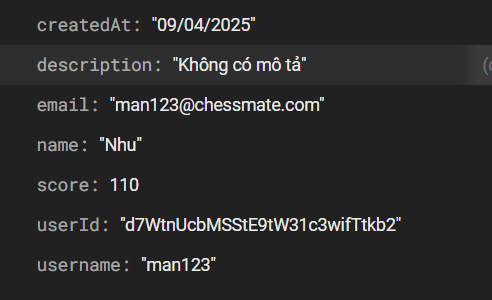
\includegraphics[width=0.9\textwidth]{img/user.png}
          \end{center}
    \item \textbf{friends:} quản lý mối quan hệ bạn bè
          \begin{center}
              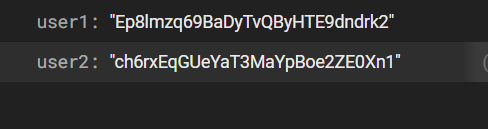
\includegraphics[width=0.9\textwidth]{img/friend.png}
          \end{center}
     \item \textbf{friends:} quản lý yêu cầu kết bạn
          \begin{center}
              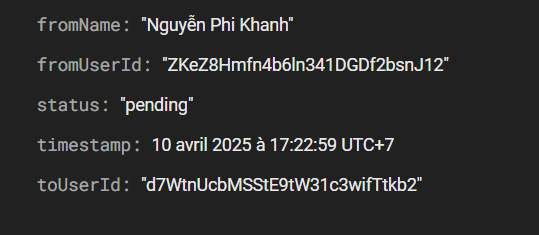
\includegraphics[width=0.9\textwidth]{img/friend_request.png}
          \end{center}
    \item \textbf{matches:} lưu thông tin các trận đấu
          \begin{center}
              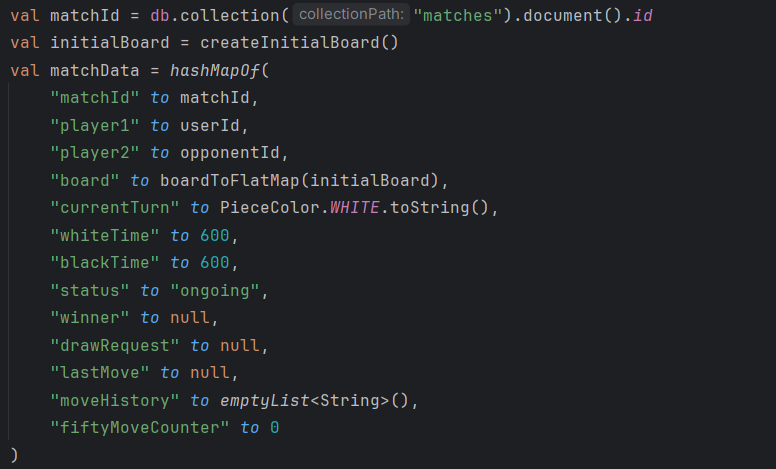
\includegraphics[width=0.9\textwidth]{img/match.png}
          \end{center}
    \item \textbf{rankings:} danh sách xếp hạng người chơi, có thể cập nhật định kỳ hoặc theo sự kiện
\end{itemize}

\subsection*{3.4. Thiết kế thuật toán chơi với AI} % Heading 2 

\justify
\noindent Ứng dụng sử dụng thuật toán Minimax kết hợp với Alpha-Beta pruning để xây dựng AI chơi cờ:

\noindent \textbf{\large \textit{Minimax:}} Thuật toán tìm kiếm theo chiều sâu, mô phỏng các nước đi và phản ứng của đối thủ, từ đó chọn nước đi tối ưu.\\

\noindent \textbf{\large \textit{Alpha-Beta pruning:}} Cải tiến của Minimax, giúp cắt bớt các nhánh không cần thiết, tăng tốc độ xử lý.\\
\noindent Độ sâu (depth) của thuật toán được điều chỉnh theo độ khó của người chơi lựa chọn.

\subsection*{3.5. Luồng hoạt động chính} % Heading 2 

\subsubsection*{3.5.1. Luồng chơi online} % Heading 3 

\begin{itemize}[label=·]
    \item Người dùng bấm "Chơi Online"
    \item Hệ thống kiểm tra phòng đang chờ
    \item Nếu có, ghép người chơi vào phòng đó; nếu không, tạo phòng mới
    \item Hai người chơi thi đấu theo lượt
    \item Khi ván đấu kết thúc, hệ thống cập nhật kết quả, lịch sử trận đấu, và điểm xếp hạng
\end{itemize}

\subsubsection*{3.5.2. Luồng thêm bạn} % Heading 3 

\begin{itemize}[label=·]
    \item Người dùng tìm kiếm tên người chơi
    \item Gửi lời mời kết bạn
    \item Người nhận xác nhận lời mời
    \item Hệ thống cập nhật mối quan hệ trong collection friends
\end{itemize}

\subsection*{3.6. Sơ đồ chức năng (Use Case Diagram)} % Heading 2 



\end{document}